\documentclass[10pt]{article}
\usepackage{neurips_2024}
\usepackage{booktabs}
\usepackage{graphicx}
\usepackage{hyperref}
\usepackage{amsmath}
\usepackage{enumitem}
\usepackage{float}

\title{Weather, Mental-Health Treatment, and Burnout Prediction}
\author{IceT Thaewanarumitkul \\ STAT 390 Final Project}
\date{}

\begin{document}
\maketitle

\begin{abstract}
This project tests whether weather variables add predictive value beyond worker, demographic, sleep, and workplace variables. I evaluate two targets: a binary mental-health treatment outcome, \texttt{sought\_treatment}, and a continuous PCA-derived \texttt{burnout\_index}. The best treatment models improve strongly over the dummy baseline, from 0.3915 weighted F1 to about 0.796. Across the controlled experiment, weather adds only a negligible improvement for treatment prediction and a small improvement for burnout-index regression. However, variable importance shows that weather has a clearer signal for \texttt{sought\_treatment}: wind gust is the third most important variable in the weather-augmented treatment model, while room temperature is much smaller in the burnout-index model.
\end{abstract}

\section{Research Question and Data}
The central research question is whether weather exposure improves prediction of mental-health and burnout-related outcomes. The project is motivated by prior research suggesting that temperature, sunlight, wind, and seasonal conditions can affect mood, depression, and performance. This project tests a narrower predictive question: do weather variables improve model performance after non-weather predictors are already included?

The project uses three data sources. The mental-health survey file provides the \texttt{sought\_treatment} target and workplace mental-health predictors. The sleep-health dataset provides sleep, work, and health variables. A weather pipeline downloads or stores state-level weather features and merges them into the modeling tables. The weather features include variables such as temperature, humidity, wind, pressure, sunlight, and related derived fields when available.

The burnout target is constructed separately with PCA. Weather variables are intentionally excluded from index construction to avoid leakage. The PCA source variables include stress, work hours, sleep quality, sleep duration, feeling rested, cognitive performance, sleep latency, wake episodes, and weekend sleep difference. Higher \texttt{burnout\_index} values represent higher burnout risk.

\section{Experimental Design}
The main experiment is a controlled ablation. For each target, I train models with non-weather predictors and then with weather-augmented predictors. The same random seed, split policy, preprocessing pipeline, and model list are used within each paired comparison. Classification uses weighted F1 as the primary metric. Regression uses $R^2$ as the primary metric.

The full experiment suite runs 22 models for each of four controlled runs: treatment without weather, treatment with weather, burnout index without weather, and burnout index with weather. Candidate models include dummy baselines, logistic and ridge models, SGD models, support-vector models, K-nearest neighbors, decision trees, random forests, extra trees, gradient boosting, histogram gradient boosting, and multilayer perceptron neural networks. Every model attempt is logged to \texttt{results/historical\_experiment\_log.csv}.

\begin{table}[H]
\centering
\small
\caption{Controlled experiment results.}
\begin{tabular}{llllrr}
\toprule
Target & Feature set & Baseline & Best model & Best & Gain \\
\midrule
\texttt{sought\_treatment} & Non-weather & 0.3915 & HistGradientBoosting & 0.7962 & +0.4047 \\
\texttt{sought\_treatment} & Weather & 0.3915 & Logistic\_C0.1 & 0.7963 & +0.4048 \\
\texttt{burnout\_index} & Non-weather & -0.0001 & HistGradientBoostingReg & 0.7938 & +0.7939 \\
\texttt{burnout\_index} & Weather & -0.0001 & HistGradientBoostingReg & 0.7958 & +0.7959 \\
\bottomrule
\end{tabular}
\end{table}

\begin{figure}[H]
\centering
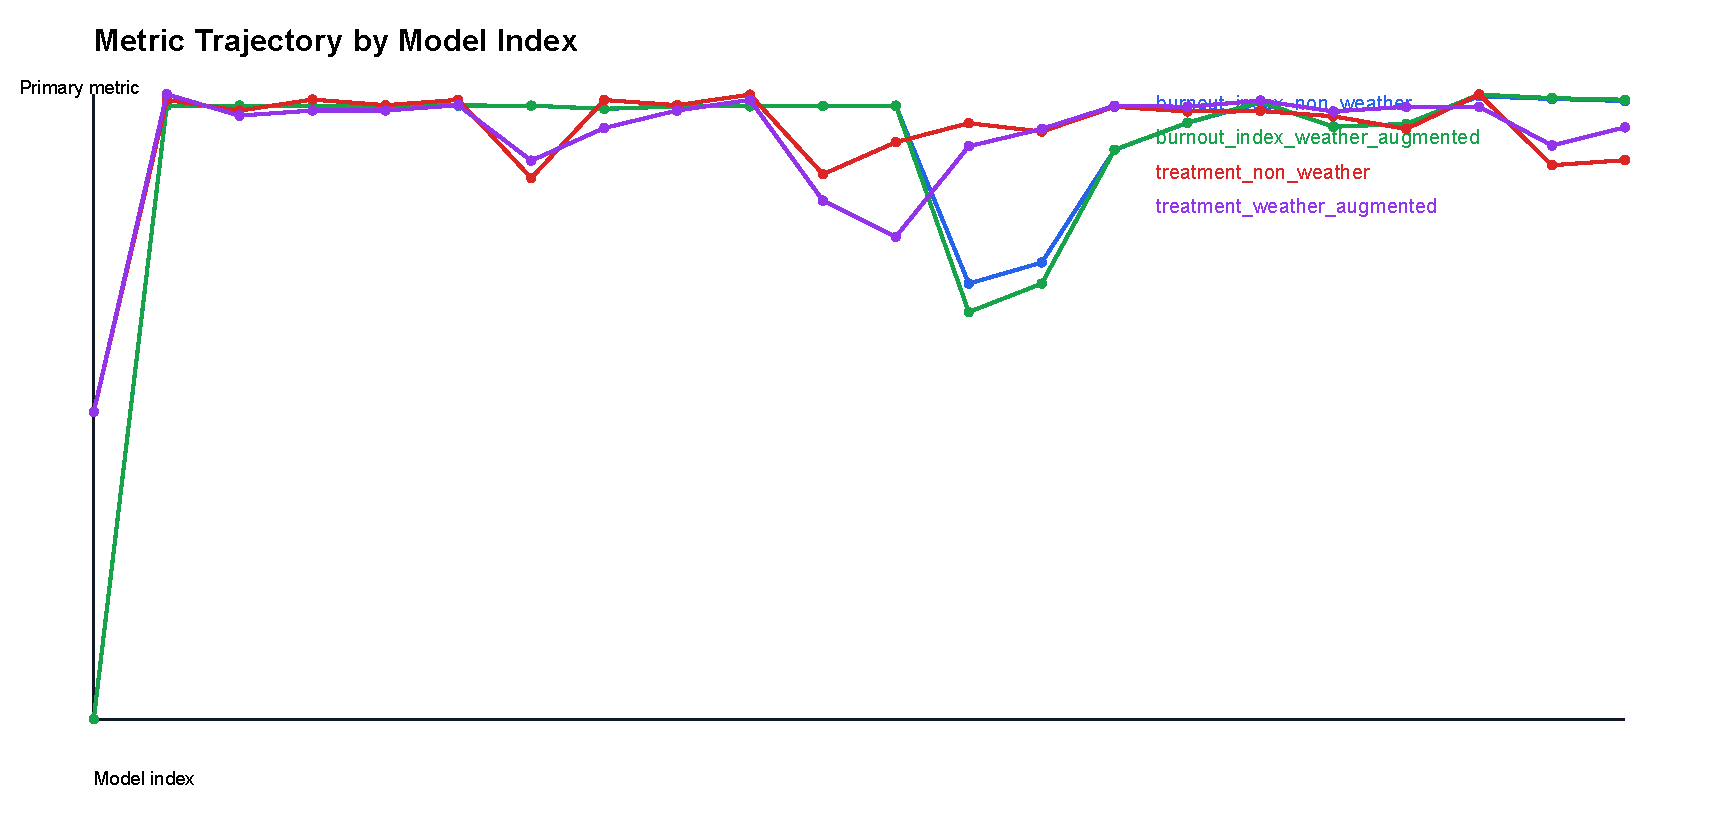
\includegraphics[width=0.92\linewidth]{metric_trajectory_plot.pdf}
\caption{Metric trajectory across the latest full experiment. Each run shows the best-performing model trajectory over model index.}
\end{figure}

\section{Results}
Both treatment models are much better than the dummy baseline. The non-weather treatment run improves from 0.3915 to 0.7962 weighted F1, and the weather-augmented treatment run improves from 0.3915 to 0.7963 weighted F1. This shows that the modeling pipeline finds a strong treatment-prediction signal. The weather-vs-non-weather difference is much smaller: weather adds only about 0.0002 weighted F1 over the best non-weather treatment model.

The weather variables are still more visible for \texttt{sought\_treatment} than for the burnout index. In the weather-augmented treatment model, the top features are family history, work interference, wind gust, mental-health consequences, and care options. Wind gust has permutation importance 0.0260, making it the strongest weather feature and the third strongest feature overall. Pressure also appears in the top ten. This supports a cautious interpretation: weather does not greatly improve treatment prediction, but weather features show some relationship to the treatment outcome.

The burnout-index models show a slightly clearer weather gain. The controlled non-weather model reaches $R^2=0.7938$, while the weather-augmented version reaches $R^2=0.7958$. A focused improvement pass with tuned histogram-gradient-boosting models improves the weather-augmented burnout result to $R^2=0.7962$. This is the best overall result, but the gain over the non-weather focused model is still small.

\begin{table}[H]
\centering
\small
\caption{Focused improvement results.}
\begin{tabular}{llllr}
\toprule
Target & Feature set & Best focused model & Metric & Value \\
\midrule
\texttt{sought\_treatment} & Non-weather & HistGB\_lr003\_leaf15\_l2 & Weighted F1 & 0.7959 \\
\texttt{sought\_treatment} & Weather & Logistic\_C0.03\_balanced & Weighted F1 & 0.7897 \\
\texttt{burnout\_index} & Non-weather & HistGBReg\_lr002\_leaf63\_l2 & $R^2$ & 0.7944 \\
\texttt{burnout\_index} & Weather & HistGBReg\_lr002\_leaf63\_l2 & $R^2$ & 0.7962 \\
\bottomrule
\end{tabular}
\end{table}

\begin{table}[H]
\centering
\small
\caption{Top weather-augmented treatment importance values.}
\begin{tabular}{lr}
\toprule
Feature & Permutation importance \\
\midrule
family\_history & 0.0726 \\
work\_interfere & 0.0563 \\
wind\_gust & 0.0260 \\
mental\_health\_consequence & 0.0259 \\
care\_options & 0.0199 \\
pressure\_hpa & 0.0055 \\
\bottomrule
\end{tabular}
\end{table}

\begin{figure}[H]
\centering
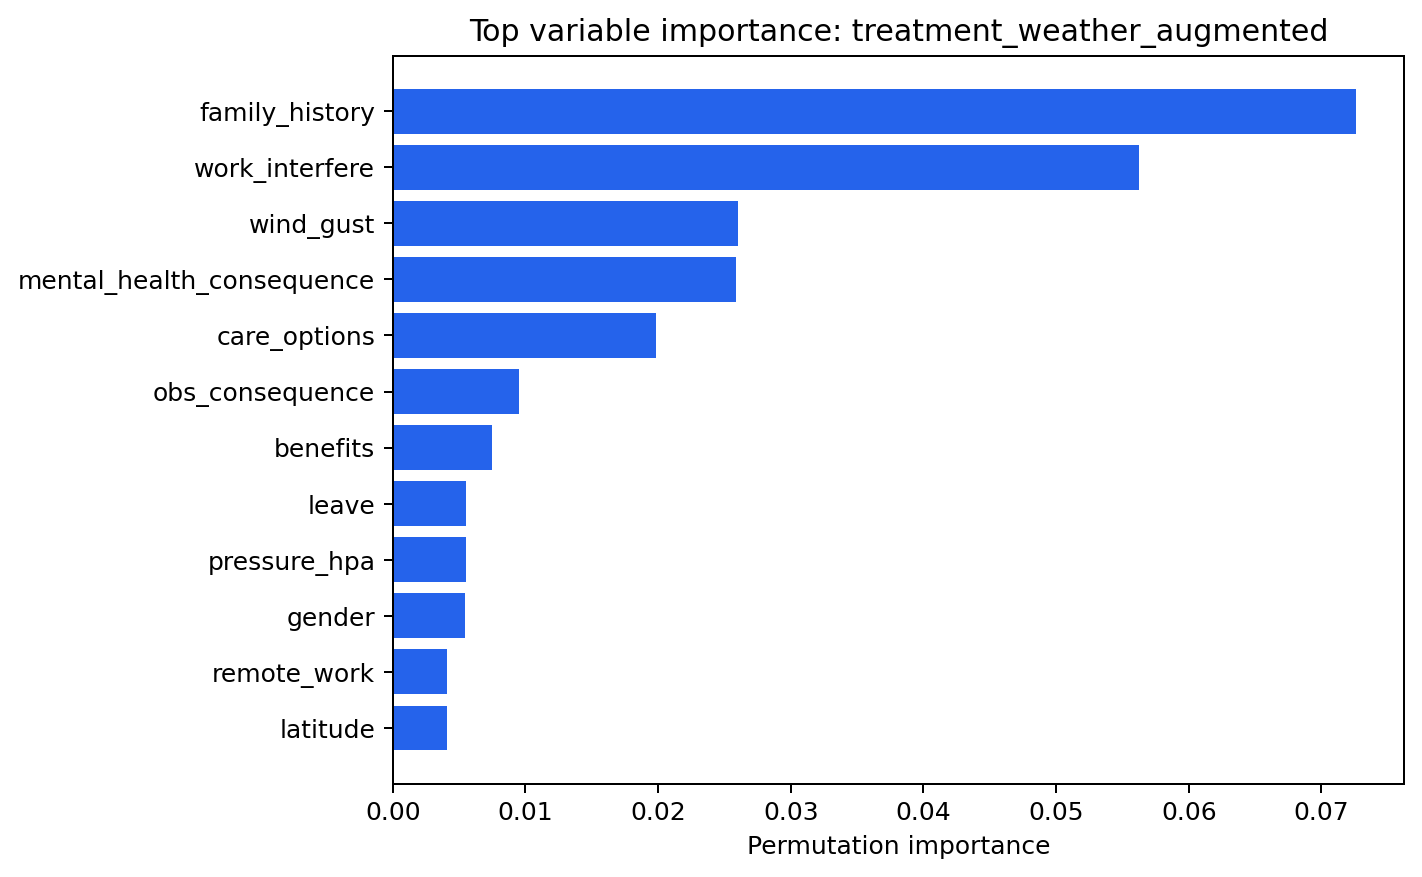
\includegraphics[width=0.49\linewidth]{../figures/treatment_weather_augmented_variable_importance.png}
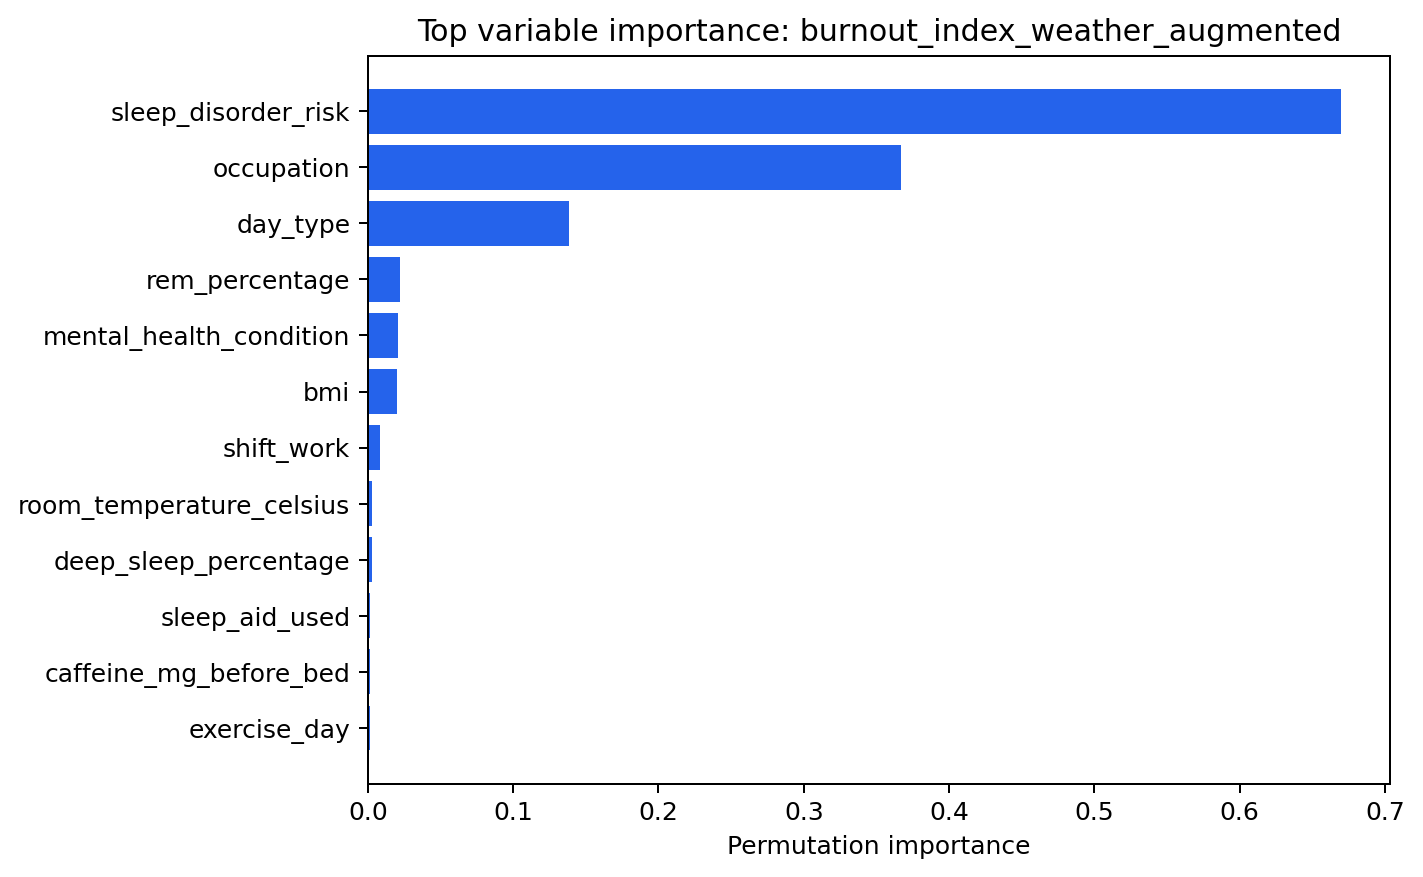
\includegraphics[width=0.49\linewidth]{../figures/burnout_index_weather_augmented_variable_importance.png}
\caption{Permutation importance for the weather-augmented treatment model (left) and burnout-index model (right). Weather is more visible in treatment prediction through wind gust and pressure, while burnout prediction is dominated by sleep and work variables.}
\end{figure}

\section{Interpretation and Limitations}
The final conclusion is cautious. Weather variables provide weak incremental predictive value in this project, especially for burnout-index regression, but they are not major predictors. The weather result does not contradict prior research that weather can affect depression or performance. Prior work may study direct causal effects, repeated daily exposure, seasonal changes, sunlight duration, or extreme weather events. This project instead asks whether weather improves prediction after strong individual, work, sleep, and health predictors are already included.

The strongest burnout predictors are sleep disorder risk, occupation, day type, REM percentage, mental-health condition, and BMI. Room temperature appears in the importance results, but its importance is much smaller than the leading sleep and work variables. This suggests weather may matter indirectly through sleep, stress, or workplace behavior, while direct weather variables add little once those mediating variables are already in the model.

The largest limitation is weather granularity. Weather is matched at broad geographic levels or through available room-temperature and season fields, not through exact personal exposure histories. More precise local weather, date-aligned exposure windows, heat-wave indicators, sunlight duration, and longitudinal observations could produce stronger weather effects. The validation design is also predictive, not causal, so the results should be interpreted as incremental model performance rather than proof of no weather effect.

\newpage
\section{Reproducibility and Deliverables}
The cleaned repository is available at \url{https://github.com/ICET2003/STAT390}. The full experiment record is stored in \texttt{results/historical\_experiment\_log.csv}, with the latest controlled matrix in \texttt{reports/experiment\_result\_matrix.csv}. The final results table is \texttt{reports/final\_results\_table.md}, and the reflection memo is \texttt{reports/reflection\_memo.md}. The latest full experiment completed 88 models with zero model failures; historical logs contain 168 total experiment rows.

The final repository is organized so that each result can be regenerated from scripts rather than manual notebook state. Data preparation, weather merging, burnout-index construction, full controlled experiments, focused improvement experiments, variable importance, and PDF report generation are all represented as scripts. The main experimental record is append-only, so older attempts are preserved while the latest result matrices and reports are regenerated for submission. This organization makes the project easier to audit: the final table summarizes the result, the historical log records how the result was reached, and the reflection memo explains what worked, what did not work, and why the weather findings should be interpreted cautiously.

\end{document}
